% Created 2023-02-03 Fri 08:38
% Intended LaTeX compiler: pdflatex
\documentclass[presentation,aspectratio=169]{beamer}
\usepackage[utf8]{inputenc}
\usepackage[T1]{fontenc}
\usepackage{graphicx}
\usepackage{grffile}
\usepackage{longtable}
\usepackage{wrapfig}
\usepackage{rotating}
\usepackage[normalem]{ulem}
\usepackage{amsmath}
\usepackage{textcomp}
\usepackage{amssymb}
\usepackage{capt-of}
\usepackage{hyperref}
\usepackage{khpreamble}
\usepackage{amssymb}
\usepgfplotslibrary{groupplots}
\newcommand*{\shift}{\ensuremath{\operatorname{q}}}
\newcommand*{\vecref}[2]{\ensuremath{^#2 \vec{#1}}}
\newcommand*{\pref}[2]{\ensuremath{^#2{#1}}}
\newcommand*{\refsys}[1]{\ensuremath{\{#1\}}}
\newcommand*{\refframe}[4]{%
\draw[->, thick, #4] (0,0) to (#1, 0) node[right]{#2};
\draw[->, thick, #4] (0,0) to (0, #1) node[above]{#3};}
\usetheme{default}
\author{Kjartan Halvorsen}
\date{\today}
\title{Pose en 2D}
\hypersetup{
 pdfauthor={Kjartan Halvorsen},
 pdftitle={Pose en 2D},
 pdfkeywords={},
 pdfsubject={},
 pdfcreator={Emacs 26.3 (Org mode 9.4.6)}, 
 pdflang={English}}
\begin{document}

\maketitle

\section{Intro}
\label{sec:orge97e38b}
\begin{frame}[label={sec:orgd476b22}]{Definiciones}
\begin{center}
\includegraphics[height=0.5\textheight]{../figures/Corke-fig2.1.a.png}

\footnotesize Peter Corke \emph{Robotics, vision and control}
\end{center}
\end{frame}


\begin{frame}[label={sec:org8aaa56b}]{Uso de sistemas de referencia en robótica}
\begin{center}
\includegraphics[height=0.65\textheight]{../figures/Corke-fig2.4.png}

\footnotesize Peter Corke \emph{Robotics, vision and control}
\end{center}
\end{frame}

\section{Pose en 2D}
\label{sec:org6a76eeb}

\begin{frame}[label={sec:org7ad32f8}]{Pose en 2D}
\begin{center}
\includegraphics[height=0.9\textheight]{../figures/2d-transform}
\end{center}
\end{frame}

\begin{frame}[label={sec:orge9197f0}]{Pose en 2D}
\begin{columns}
\begin{column}{0.3\columnwidth}
\begin{center}
\includegraphics[height=0.6\textheight]{../figures/2d-transform}
\end{center}
\end{column}

\begin{column}{0.7\columnwidth}
\footnotesize

El vector \(\vec{x_B}\) en sistema \refsys{A}:
\[ \vec{x_B} = \cos\theta \vec{x_A} +\sin\theta\vec{y_A} =
\begin{bmatrix}\vec{x_A} & \vec{y_A} \end{bmatrix} \begin{bmatrix} \cos\theta\\\sin\theta \end{bmatrix}\]
\[ \vecref{x_B}{A} = \cos\theta \vecref{x_A}{A} +\sin\theta\vecref{y_A}{A} = \begin{bmatrix} \cos\theta\\\sin\theta \end{bmatrix}\]

\pause
El vector \(\vec{y_B}\) en sistema \refsys{A}: \[ \vec{y_B} = -\sin\theta \vec{x_A} +\cos\theta\vec{y_A} =
\begin{bmatrix}\vec{x_A} & \vec{y_A} \end{bmatrix} \begin{bmatrix} -\sin\theta\\\cos\theta \end{bmatrix}\]
\[ \vecref{y_B}{A} = -\sin\theta \vecref{x_A}{A} +\cos\theta\vecref{y_A}{A} = \begin{bmatrix} -\sin\theta\\\cos\theta \end{bmatrix}\]

\pause

El punto \(P\) en sistema \refsys{A}: \(p_A = O_A + v_A\), donde:

\[ \vec{v}_A = \vec{t}_{ab} + \vec{v}_B = \vec{t}_{ab} + \pref{p}{B}_x \vec{x_B} + \pref{p}{B}_y \vec{y_B}\]
\pause
\[\vecref{v_A}{A} &= \vecref{t_{ab}}{A} + \pref{p}{B}_x \vecref{x_B}{A} + \pref{p}{B}_y \vecref{y_B}{A}
= \vecref{t_{ab}}{A} + \begin{bmatrix} \vecref{x_B}{A} & \vecref{y_B}{A} \end{bmatrix} \begin{bmatrix} \pref{p}{B}_x\\ \pref{p}{B}_y \end{bmatrix}\]
\end{column}
\end{columns}
\end{frame}




\begin{frame}[label={sec:org7c88a10}]{Pose en 2D}
\begin{columns}
\begin{column}{0.3\columnwidth}
\begin{center}
\includegraphics[height=0.6\textheight]{../figures/2d-transform}
\end{center}
\end{column}

\begin{column}{0.7\columnwidth}
\footnotesize


El punto \(P\) en sistema \refsys{A}: \(p_A = O_A + v_A\), donde:

\[ \vec{v}_A = \vec{t}_{ab} + \vec{v}_B = \vec{t}_{ab} + \pref{p}{B}_x \vec{x_B} + \pref{p}{B}_y \vec{y_B}\]
\[\vecref{v_A}{A} &= \vecref{t_{ab}}{A} + \pref{p}{B}_x \vecref{x_B}{A} + \pref{p}{B}_y \vecref{y_B}{A}
= \vecref{t_{ab}}{A} + \begin{bmatrix} \vecref{x_B}{A} & \vecref{y_B}{A} \end{bmatrix} \begin{bmatrix} \pref{p}{B}_x\\ \pref{p}{B}_y \end{bmatrix}\]

\pause

\[ = \vecref{t_{ab}}{A} + \begin{bmatrix} \cos\theta & -\sin\theta\\\sin\theta & \cos\theta \end{bmatrix} \begin{bmatrix} \pref{p}{B}_x\\ \pref{p}{B}_y \end{bmatrix}\]
\end{column}
\end{columns}
\end{frame}

\begin{frame}[label={sec:org0885944}]{Ejemplo}
\begin{columns}
\begin{column}{0.6\columnwidth}
\begin{center}
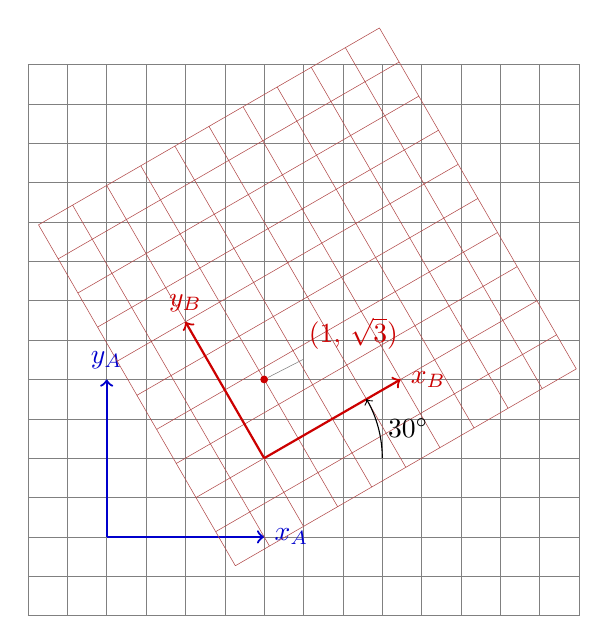
\begin{tikzpicture}[scale=0.5]

\def\xxa{4}
\def\yya{4}
\def\bx{4}
\def\by{2}
\def\thth{30}
\pgfmathsetmacro{\cth}{cos(\thth)}
\pgfmathsetmacro{\sth}{sin(\thth)}
\pgfmathsetmacro{\xxb}{\cth*(\xxa-\bx) + \sth*(\yya-\by)}
\pgfmathsetmacro{\yyb}{-\sth*(\xxa-\bx) + \cth*(\yya-\by)}

\draw[step=1cm, gray, very thin] (-2, -2) grid (12,12);

\refframe{4}{$x_A$}{$y_A$}{blue!80!black}

\begin{scope}[xshift = \bx cm, yshift=\by cm, rotate=\thth]
  \draw[step=1cm, red!40!gray, very thin] (-2, -2) grid (8,8);
  \refframe{4}{$x_B$}{$y_B$}{red!80!black}
  \node[red!80!black, pin={[red!80!black] 30:{($1$, $\sqrt{3}$)}}, circle, fill, inner sep=1pt] at (\xxb cm, \yyb cm) {};
\end{scope}

\draw[->] (7, 2) arc[radius=3cm, start angle=0, end angle=30] node[right, pos=0.5] {$30^\circ$};

%\node[red!80!black, pin=30:{}, circle, fill, inner sep=1pt] at (\xxa cm, \yya cm) {};
\end{tikzpicture}
\end{center}
\end{column}


\begin{column}{0.4\columnwidth}
\small
Determine la matriz de rotación \(R_{ab}\) y la translación \(t_{ab}\) que definen la transformación entre \refsys{B} y \refsys{A}. Verifique que
\begin{align*}
^Ap &= \begin{bmatrix}4\\4\end{bmatrix} = R_{ab} ^Bp + t_{ab}\\
&=  R_{ab}\begin{bmatrix}1\\\sqrt{3}\end{bmatrix} + t_{ab}
\end{align*}
\end{column}
\end{columns}
\end{frame}

\begin{frame}[label={sec:orgcdc7097}]{Ejercicio}
\begin{columns}
\begin{column}{0.6\columnwidth}
\begin{center}
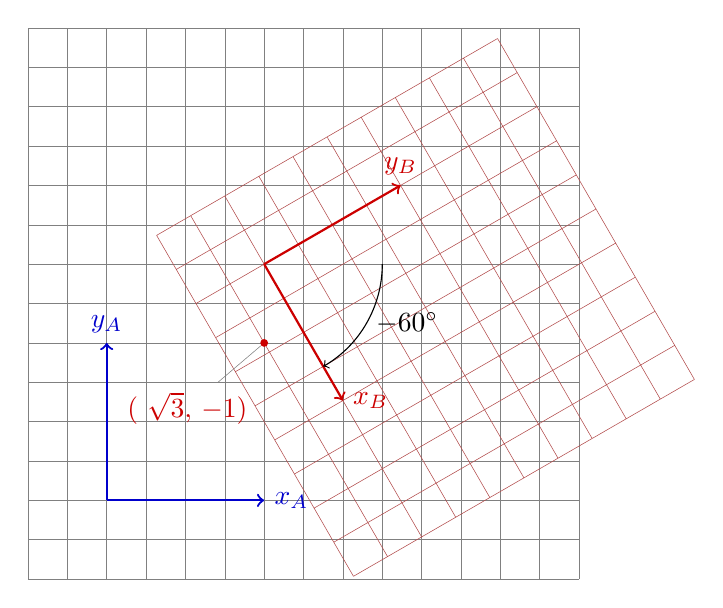
\begin{tikzpicture}[scale=0.5]

\def\xxa{4}
\def\yya{4}
\def\bx{4}
\def\by{6}
\def\thth{-60}
\pgfmathsetmacro{\cth}{cos(\thth)}
\pgfmathsetmacro{\sth}{sin(\thth)}
\pgfmathsetmacro{\xxb}{\cth*(\xxa-\bx) + \sth*(\yya-\by)}
\pgfmathsetmacro{\yyb}{-\sth*(\xxa-\bx) + \cth*(\yya-\by)}

\draw[step=1cm, gray, very thin] (-2, -2) grid (12,12);

\refframe{4}{$x_A$}{$y_A$}{blue!80!black}

\begin{scope}[xshift = \bx cm, yshift=\by cm, rotate=\thth]
  \draw[step=1cm, red!40!gray, very thin] (-2, -2) grid (8,8);
  \refframe{4}{$x_B$}{$y_B$}{red!80!black}
  \node[red!80!black, pin={[red!80!black] -100:{( $\sqrt{3}$, $-1$)}}, circle, fill, inner sep=1pt] at (\xxb cm, \yyb cm) {};
\end{scope}

\draw[->] (7, 6) arc[radius=3cm, start angle=0, end angle=-60] node[right, pos=0.5] {$-60^\circ$};

%\node[red!80!black, pin=30:{}, circle, fill, inner sep=1pt] at (\xxa cm, \yya cm) {};
\end{tikzpicture}
\end{center}
\end{column}

\begin{column}{0.4\columnwidth}
Determine la matriz de rotación \(R_{ab}\) y la translación \(t_{ab}\) que definen la transformación entre \refsys{B} y \refsys{A}. Verifique que
\begin{align*}
^Ap &= \begin{bmatrix}4\\4\end{bmatrix} = R_{ab} ^Bp + t_{ab}\\
&=  R_{ab}\begin{bmatrix}\sqrt{3}\\-1\end{bmatrix} + t_{ab}
\end{align*}
\end{column}
\end{columns}
\end{frame}


\begin{frame}[label={sec:orge675d08}]{Programar}
\end{frame}
\end{document}